\chapter[My Reflections on Professor GR]{My Reflections on\\ Professor GR}\label{chap12}

\Authorline{M V Satyanarayana\footnote[*]{Email: \url{0407mvs@gmail.com}}}

\authinfo{Department of Physics, IIT Madras, Chennai - 600036}

I first came to know about Professor G. Ramachandran (affectionately known as GR) in 1980, when I joined the Institute of Mathematical Sciences (IMSc) as a research scholar. My advisor Professor T. S. Santhanam (TSS) `introduced' me to GR. In this article, a humble salutation of my Shraddhanjali to his memory, I wish to record my experiences with him, by highlighting on a few of his qualities.

My advisor TSS, had put me on a Clebsch-Gordan program involving angular momentum in finite dimensional quantum mechanics, a topic on which he had written several papers during 1975--1980. I decided to learn the basics of the quantum theory of angular momentum and I looked for the famous books on the topic by M. E. Rose and A. R. Edmonds. Surprisingly, these books were not available in the library of IMSc! There was this 1962 Matscience Report: 2, on the quantum theory of angular momentum, a lecture notes of GR. This report was repeatedly re-cyclostyled as there was a good demand for it, in India and abroad. I could gauge that GR was held with admiration and respect by TSS and other faculty members of IMSc.

During my visit to Mysore in 1981, I met GR for the first time - thanks to my good friend K. S. Mallesh (KSM), who was then, one of several research scholars of GR. I have met GR many times till 2018. It has always been an illuminating experience to discuss Physics with him. He had a heuristic way to look into a problem and tell what kind of Physics would emerge out. Then, he would formulate the mathematical equations and then proceed to obtain the solutions. I have had clear physical pictures emerging from discussions with him on several instances. His students and others could see his fluency in analytical methods. Also, he used to come out with several appropriate anecdotes, told in an inimitable style about various Physicists and his experiences during his Ph.D. days in 1957--1962 at the Department of Physics, the University of Madras in the A. C. College Campus, and his subsequent stay at IMSc.

\begin{enumerate}
\itemsep=0pt
\item In my opinion, he endeared himself to students and others with his genuine love for Theoretical Physics, the way he elaborated the subject in his classes and discussions, the kind of unadulterated concern he had for students, etc. He was very strong in Mathematical Physics and that aspect was well cherished and loved by those students who had inclination towards Theoretical Physics. In fact, the Department of Physics of the Mysore University had a robust program in Theoretical Physics. I was envious of KSM and his co-researchers, since they had a very good syllabus in Theoretical Physics specialization and they were taught by such brilliant Professors like K. N. Srinivasa Rao, GR and Gopal Rao, whereas, we at IMSc were resentful that we were grappling to learn the subject on our own! Many of KSM's friends became my friends too. I remember a talk I gave to GR and his students in his office room in a very lively atmosphere and the kind of discussions that ensued. GR had a way of asking questions to a greenhorn like me, and I felt encouraged and happy. GR was heading a group of young researchers and M.Sc.\ students who were zealots of Theoretical Physics and that way he was presiding over a school in a university outside such institutions like TIFR, IMSc, etc.\ Later many of his students became distinguished faculty members and active researchers in several Departments of Physics. Like GR, many of his students became sincere and committed teachers.
\item GR had an interesting way of looking at things and events and he used to narrate anecdotes in a humorous way without any malice or hatred. With stentorian voice and boisterous laughter, he was enthusiastic of recounting reminiscences about well-known scientists like Homi Bhabha, Murray Gell-Mann, Schiff, P. A. M. Dirac, C. V. Raman, Robert Marshak, G. N. Ramachandran, C. R. Rao, Alladi Ramakrishnan and several others, who had visited the A. C. College Campus and IMSc in his Madras days. Many such anecdotes were actually told with admiration and respect towards those great people. He along with Professor V. Devanathan, the former Head of the Department of Nuclear Physics, and many others were the members of the actual `core group' - (about which, I only hope a research scholar of that group would record their experiences in those halcyon days) - which preceded the creation of IMSc - and, its members self-taught themselves and each other, topics like Nuclear Physics, Particle Physics, etc., then, new to the Madras University. It should have been a very vibrant and salubrious atmosphere filled with hope and joy, learning Blatt and Weisskopf and Feynmann diagrams on their own and applying what they learnt to various nuclear reactions by hand-calculating the cross-sections with the classical Facit machines and slide rules in those pre-computer days in the city of Madras and getting their results published in internationally refereed journals! The creation of IMSc owes much to the scientific contributions of young researchers who were drawn to Professor Alladi Ramakrishnan during 1955--1962. Almost all members of this `core group' became very active professional Physicists in India and abroad.
\item There is another side of GR which I happen to like very much, that is, his devotion to his thesis advisor Professor Alladi Ramakrishnan (AR), the founder director of IMSc. GR, though had to leave IMSc in mid 1960's, his allegiance to his teacher was something, which I admire. In early 1980's, AR was on a visit to Mysore and I was there at that time. AR was invited to give a talk in the Department of Physics, University of Mysore. I could see the humbleness with which GR was talking to AR, and I for one appreciate and commend this traditional teacher-student relationship. After the talk, it was already 7.00 p.m or so, and for an hour or so, GR went on narrating with love and affection about his teacher and his days with him in the AC College and IMSc.
\item There is another aspect of GR, which was very striking to me in those days and now too. He was very orthodox with respect to his food habits, nithya pooja and anushtana, etc. He would not partake food prepared outside his home kitchen. At the same time, he was a very generous host to one and all, especially to his students. It was very common that his students go to his place for discussions in evenings, and these discussions continue beyond 8.00 p.m or so, and they were generously fed before they left.
\eject
\item Later in 1995, I became a Reader in the Department of Physics, Mangalore University, a university in Karnataka. I went to take blessings from GR and seek his suggestions and counsel. I was somewhat worried and concerned as I was not used to the circumstances and conditions in a university. He gave a picture of the kind of atmosphere in a university set up and his words of advice were very useful to me and I shall remain thankful to him for that. I must mention that I made it a practice to send my manuscripts prior to publication to him for his perusal and comments. I am benefited by his comments and words of encouragement for which I am indebted to him. I met him for the last time in early 2018 and he was as light-hearted and exuberant as he used to be in his heydays at Mysore. I think that he was requested by some enthusiasts to deliver lectures on quantum mechanics, nuclear physics, etc. About an year ago, I received a copy of his lecture notes prepared in an informal style. If, GR had written a couple of text- books or monographs, laced with insights and interpretations, what an immense help it would have been, especially to the learners in particular and also to the teachers! At a personal level, he was like a reassuring and benevolent elder brother, on whom I could count on for proper directions.
\end{enumerate}
\vskip .2cm

\centerline{\includegraphics[scale=2.5]{authorsphotos/Prof_M_V_Satyanarayana.eps}}
\bigskip

\noindent
\textbf{Prof.\ M. V. Satyanarayana} obtained Ph.D. from The Institute of Mathematical Sciences in 1987 under the supervision of Prof.\ T. S. Santhanam. He was a Post-Doctoral Fellow from 1987 to 1989 at University of Arkansas, Fayetteville, USA and later at IIT Madras for brief periods. He joined Mangalore University as a Reader in 1992 and moved to IIT Madras in 1995. He is currently a Professor in the Department of Physics, IIT Madras.
